\section{Introduction}

	Astrophysical and cosmological observations present evidence that 27\% of the mass-energy of the Universe is made out of Dark Matter (DM), a non-luminous, non-baryonic and non-relativistic particle, though the nature of this particle is yet unknown~\cite{Harvey1462}. While several types of new DM candidate raise from many theories, the most prominent one is the Weakly Interacting Massive Particles(WIMPs)~\cite{Bertone:2010zza}. Many  direct detection experiments attempt to measure the rare scattering of WIMPs from target nucleus. Although some experiment see an excess for WIMPs in the mass range of 6-30 GeV/$C^2$~\cite{DAMA,COGENT,CDMSlite,CREST}, these results are in tension with other experiments~\cite{xe100_run_combination,PANDAX,LUXnew}.
	
	 Typically the standard calculation for WIMP-nucleon scattering simplifies the type of interaction to Spin Independent (SI) and Spin Dependent (SD) interactions~\cite{LEWIN}, however these are not the only possible types of interactions. In recent years an Effective Field Theory (EFT) approach that takes into account all leading-order and next-to-leading order operators that emerge from an effective Lagrangian describing the WIMP-nucleus interaction has been developed ~\cite{Fitzpatrick:2012ib,Anand:MathTools,Fitzpatrick:MathTools}. In this framework new operators which come from different type of nuclear responses are introduced along with the standard SI and SD ones. The parametrization of the fourteen operators $\mathcal{O}_i$ is listed in Eq.~\ref{eq:OpDef} and follows the convention from~\cite{Anand:MathTools}. The operators dependence explicitly on 4 quantities: $\vec{v}^{\perp}$, the relative velocity between the WIMP and the nucleon, $\vec{q}$, the momentum transfer, and the WIMP and nucleon spin $\vec{S}_\chi$ , $\vec{S}_N$. Notice that $\mathcal{O}_2$ is not treated as it cannot be obtained from a relativistic operator at leading order.
	 
	    Unlike The formally studied types of interaction (SI,SD) which are not suppressed when $\vec{q} \rightarrow 0$ and most of their interaction rate will be in low energies recoils, some of the new operators depend explicitly on $\vec{q}$ therefore their interaction rate is suppressed with $\vec{q}$ and peaks at higher energies than previously looked in direct detection experiments ($< 43$ keV), and hence could not be treated before see Fig. ~\ref{fig:dRdE}.
	    
	    Another assumption that can be relaxed is that WIMP should scatter elastically, however there are models in which the incoming and outgoing WIMPs have different mass states ~\cite{InelasticIntro}. In the case where the outgoing state is more massive than the incoming state the event rate at low recoil energies can again be suppressed, hence analyses which apply an upper energy bound lose sensitivity to these types of interactions. Recently an inelastic adaptation of the EFT operator framework discussed above was developed~\cite{InelasticMath}. The operators presented in~\ref{eq:OpDef} are modified such that $\vec{v}^\perp_{inelastic} = \vec{v}^\perp_{elastic} +\frac{\delta}{\vert{\vec{q}}\vert^2}\vec{q}$. \RanComment{We should add here the dependency of $v_{min}$ on $\delta$}      
	    
	    In this paper, motivated by both these extensions of the standard WIMP framework, we report on an analysis extending the energy range up to 240keV for the first time in \Xehund\ experiment, and present exclusion limits on all operators for both the elastic and the inelastic WIMP cases.     

\begin{equation} \label{eq:OpDef}
\begin{split}
&\mathcal{O}_1 = 1_{\chi} 1_N  \\
%&\mathcal{O}_2 = (v^{\perp})^2 \\
&\mathcal{O}_3 = i\vec{S}_N\cdot (\frac{\vec{q}}{m_N}\times\vec{v}^\perp) \\
&\mathcal{O}_4 = \vec{S}_{\chi}\cdot \vec{S}_N \\
&\mathcal{O}_5 = i\vec{S}_{\chi}\cdot (\frac{\vec{q}}{m_N}\times\vec{v}^\perp) \\
&\mathcal{O}_6 = (\vec{S}_{\chi} \cdot \frac{\vec{q}}{m_N})(\vec{S}_N \cdot \frac{\vec{q}}{m_N}) \\
&\mathcal{O}_7 = \vec{S}_N \cdot \vec{v}^\perp \\
&\mathcal{O}_8 = \vec{S}_{\chi} \cdot \vec{v}^\perp \\
&\mathcal{O}_9 = i\vec{S}_{\chi} \cdot(\vec{S}_N \times \frac{\vec{q}}{m_N}) \\
&\mathcal{O}_{10} = i\vec{S}_N \cdot (\frac{\vec{q}}{m_N}) \\
&\mathcal{O}_{11} = i\vec{S}_{\chi} \cdot (\frac{\vec{q}}{m_N}) \\
&\mathcal{O}_{12} = \vec{S}_\chi \cdot (\vec{S}_N \times \vec{v}^\perp) \\
&\mathcal{O}_{13} = i(\vec{S}\chi \cdot \vec{v}^\perp)(\vec{S}_N \times \frac{\vec{q}}{m_N})\\
&\mathcal{O}_{14} = i(\vec{S}_\chi \times \frac{\vec{q}}{m_N})(\vec{S}_N \cdot \vec{v}^\perp) \\
&\mathcal{O}_{15} = -(\vec{S}_\chi \times \frac{\vec{q}}{m_N})[(\vec{S}_N \times \vec{v}^\perp)\cdot \frac{\vec{q}}{m_N}]
\end{split}
\end{equation}

Each operator is present independently for protons and neutrons at the WIMP-nucleon EFT level, though UV models of course can correlate these couplings. The full EFT thus has 28 coupling parameters plus the WIMP mass, and, in the inelastic case, a mass splitting $\delta$. The parameter space is thus too large to explore in full, so we take a similar approach to the SI/SD case and characterize the experimental limit by assuming only one active operator at a time, with the coupling to protons and neutrons for that operator set equal (the isoscalar case). However, to facilitate the full exploitation of these results by the community, we provide in supplementary material a set of tools for converting any theoretical recoil spectrum $\mathrm{d}R/\mathrm{d}E$ into an accurate signal prediction for our analysis, as well as a simplified likelihood lookup table which can be used to set a mildly conservative but quite accurate limit on arbitrary models in the full EFT parameter space, or indeed any other particle dark matter model for which one has the expected recoil spectrum. (TODO, obviously this appendix and toolset doesn't exist yet, but I think we should do it.)
	        	       
%  \begin{itemize}
%  \item Motivation: dark matter, theoretical possibility of high energy recoil events. Mention some specific models, maybe inelastic scattering also.
%  \item Theoretical background on EFT operators, inc. motivation (e.g. possibility to reconcile limits vs possible signals in other experiments, model-independent approach to constraining exotic models)
%  \item (if we do it) Theoretical background on inelastic scattering kinematics.
%  \item Motivating example plots of recoil spectra/signal models (e.g. Fig. \ref{fig:dRdE}). Also discuss the lower electronic recoil background at these higher recoil energies, which improves the analysis sensitivity beyond what would be expected from the raw increase in predicted event rate (At least I presume so, need to estimate this perhaps. I think we can say something like this; the standard analysis signal region has a signal acceptance of maybe 50\% since it cuts the nuclear recoil band about in half, whereas for us it is almost 90\% since there is good separation between ER and NR bands. So for say O3 (either mass) we expect about twice as many events due to the extended signal region, with twice the acceptance in the new high PE region. So overall I guess it is roughly a factor of 3 improvement in total signal rate, and similar for the sensitivity. In fact from the proper sensitivity estimates the improvement is a little better than that, but this gives a rough idea where the improvement comes from.).
% \end{itemize}


\begin{figure}[h!]
\centerline{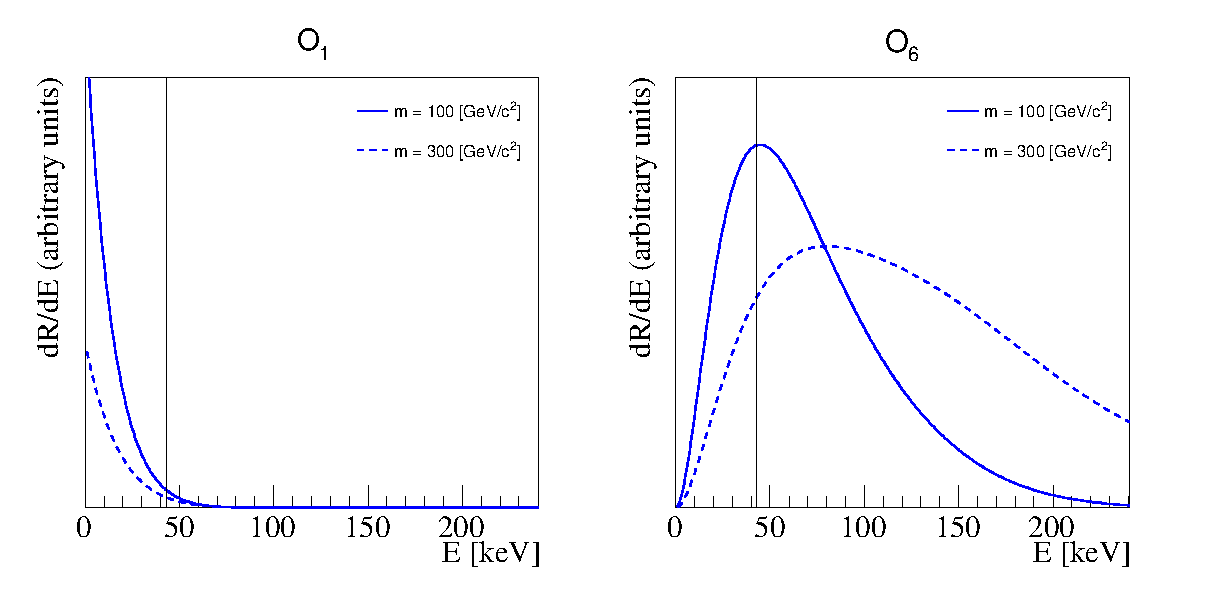
\includegraphics[width=1.\linewidth]{Figures/drdeO1O6.eps}}
\caption{Example EFT recoil spectra for elastic scattering of spin-$1/2$ WIMPs on Xenon nuclei (weighted according to the isotope abundances in the XENON100 experiment). Left(right) shows the predicted spectra for EFT operate $\mathcal{O}_1$($\mathcal{O}_6$). The normalization is controlled by the coupling coefficient of each EFT operator and the experimental exposure (left arbitrary in this figure). The solid vertical line at 43 keV shows the approximate division between the two signal regions used in this analysis (30 PE in cS1). As shown, the standard SI ($\mathcal{O}_1$) spectrum is concentrated mainly in the already explored energy region. However, some EFT operators, for certain WIMP masses, predict a significant fraction of recoil events above the upper energy cut used in the standard spin-independent analysis, motivating an extension of this cut. The highest recoil energy shown in the plots, 240 keV, roughly corresponds to the extended $cS1$ cut of 180 PE used in this analysis.}
\label{fig:dRdE}
\end{figure}

\section{The \Xehund\  Detector}
The \Xehund\ detector is a cylindrical %30\,cm~height, 30\,cm~diameter, 
dual-phase (liquid and gas) xenon time projection chamber (TPC). It is installed at the Laboratori Nazionali del Gran Sasso (LNGS) in Italy
and hosts 161\,kg of liquid xenon (LXe), of which 62\,kg perform as active target ~\cite{xe100_instr2012}. 
The detector consists of a total of 178~1-inch square Hamamatsu R8520-AL photomultiplier tubes (PMTs) employed in two arrays, one in the gas phase at the top of the TPC,
the other at the bottom, immersed in LXe. 

A particle interacting with the LXe deposits energy that creates both excited and ionized molecular states. De-excitation of these excited molecular states induce a prompt scintillation signal ($S1$), while 
electrons from ionization processes are drifted in an electric field of $530$V/cm towards the liquid-gas interface where they are extracted using larger electric field of $\sim12$kV/cm. 
These electrons generate a proportional scintillation, which is called $S2$. The spatial distribution of the $S2$ signal on the top PMT array, together with the time difference between $S1$ and $S2$ provides the X-Y and Z coordinates of the interaction, respectively,and thus a 3D position reconstructions is achieved.
%determines the X-Y position, while the time difference between the two signals gives the z-coordinate, and thus a 3D position reconstructions is achieved.

Interactions in different positions cover different solid angles with respect to the PMT array, which leads to a position-dependent S1 signal, at the same time warping of the top meshes and the absorption of electrons by residual impurities lead to a position-dependent S2 signal. To take into account these effects a correction is applied based on a light collection efficiency (LCE) map. The corrected signals (cS1,cS2) are spatially independent and uniform to all interactions~\cite{xe100_instr2012}.

The $S2/S1$ ratio is known to differ between nuclear recoil (NR) and electronic recoil (ER) interactions~\cite{}, thus used as  discriminating variable between a WIMP signal and ER background.
The logarithm of this ratio, $log(cS2/cS1)$ is referred later in the text as the $y$ discriminating variable.
% between ER background coming from $\gamma$, $\beta$ and NR signal coming from a WIMP. 

